% 基本群的计算
\pentry{基本群\upref{HomT3},可缩空间\upref{HomT2},群的自由积\upref{FrePrd}}

%基本完成

虽然把各阶同伦群都考虑进去以后可以很详细地刻画空间的伦型,但是高阶同伦群大多极其难计算.本节简单介绍一阶同伦群,即基本群的计算方法.

\subsection{基本群计算定理}

我们列举一些方便用于计算基本群的定理如下.

\begin{theorem}{积空间的基本群}
给定拓扑空间$X$和$Y$,则$\pi_1(X\times Y)=\pi_1(X)\times\pi_1(Y)$.
\end{theorem}
%需要附证明吗?直观来看这个定理很显然,证明无非就是严格把直觉描述清楚.

\begin{theorem}{Seifert-van Kampen定理}
设拓扑空间$X$可以被它的两个开集$U_1$和$U_2$覆盖,即$X=U_1\cup U_2$;若$U_1$,$U_2$和$U_1\cap U_2$都是道路连通空间,取$U_1\cap U_2$中一个点作为基点来构造各空间的基本群.设$f_i:U_1\cap U_2\rightarrow U_i$为恒等嵌入,即$\forall x\in U_1\cap U_2, f_i(x)=x\in U_i$.如果用$f_i$来定义$\pi_1(U_1\cap U_2)$到$\pi_(U_i)$上的同态,那么有:$\pi_1(X)=\pi_1(U_1)*_{\pi_1(U_1\cap U_2)}\pi_1(U_2)$.
\end{theorem}

Seifert-van Kampen定理难以简洁表达,不过如果能充分理解\textbf{群的自由积}\upref{FrePrd},应该容易理解该定理.不过,我们可以考虑该定理的弱化版本,此版本用处也很广泛:

\begin{theorem}{弱化版Seifert-van Kampen定理}
设拓扑空间$X$可以被它的两个开集$U_1$和$U_2$覆盖,并且$U_1\cap U_2$是单连通(\autoref{HomT3_ex1}~\upref{HomT3})的,那么有$\pi_1(X)=\pi_1(U_1)*\pi_1(U_2)$.
\end{theorem}

除此之外,我们在\textbf{可缩空间}\upref{HomT2}中提到的形变收缩也能用于大大简化基本群的计算.

\begin{theorem}{形变收缩核的同伦}\label{HomT5_the1}
给定拓扑空间$X$.如果$f:X\rightarrow A\in X$是一个形变收缩,且$A$是其收缩核,那么$X\cong A$.
\end{theorem}

证明很简单,由形变收缩的定义可知,$f:X\rightarrow A$和$1_X:A\rightarrow X$是彼此的同伦逆;$1_X$是$X$到自身的恒等映射,由于此处将其限制在$A$上,也可以记为$1_A=1_X|_A$.

\autoref{HomT5_the1} 很好地展示了同胚和同伦的区别:如果存在一个形变收缩,把拓扑空间压成更低维度的情况,比如将烟卷压成圆环,那么收缩前后的空间是同伦的,但它们由于维度不同,就不会同胚.

\begin{theorem}{锥空间的基本群}
设$X$是任意非空的拓扑空间,则$\pi_1(\widetilde{C}X)=\{e\}$,即为只有一个元素的平凡群.
\end{theorem}

锥空间的基本群总是平凡群,也就是说所有回路都是保基点同伦的.这是因为,首先锥空间一定是道路连通空间,因此基点可以任意选择,不妨选为锥顶点;其次,任何一条回路都可以通过各点沿着锥空间的$I$分量连续地收缩到锥顶点上,从而和恒等于锥顶点的回路同伦.



\subsection{基本群计算实例}

\pentry{复数\upref{CplxNo},覆叠空间\upref{CovTop}}

$S^1$是用于构建许多拓扑空间的伦型的原料,因此严格证明$S^1$的基本群非常重要.\autoref{HomT5_ex2} 提供了严格证明的大体思路,限于篇幅,只能由有兴趣的读者自行补充细节了.

\begin{example}{$S^1$的基本群}\label{HomT5_ex2}
将$S^1$看成复平面上的单位圆$\{\E^{2\pi\I t}\in\mathbb{C}|t\in\mathbb{R}\}=\{x+y\I\in\mathbb{C}|x=\cos{2\pi t}, y=\sin{2\pi t}\}$.取通常的实度量空间$\mathbb{R}$,建立映射$p:\mathbb{R}\rightarrow S^1$,其中$p(t)=\E^{2\pi\I t}$,则$p$是一个覆叠映射.

把$S^1$看成$\mathbb{R}$的商拓扑空间,其中等价关系$\sim$为:$x\sim y\iff \abs{x-y}\in\mathbb{Z}$,即把实数轴绕到圆上.对于圆周上任意一个点$\E^{2\pi\I t_0}$,可以取典范邻域$U_{t_0}=\{\E^{2\pi\I t}|t\in(t_0-1/4, t_0+1/4)\}$.这个典范邻域中$1/4$的选择是任意的,换成任何小于$1/2$的正数也可以,我们只需要用该典范邻域来说明接下来定义的提升映射$\tilde{f}$是唯一的.

取$S^1$的基点为$p(0)=1$,设$S^1$中有一条道路$f:I\rightarrow S^1$.我们可以把$f$\textbf{提升}为$\mathbb{R}$中的道路$\tilde{f}:I\rightarrow\mathbb{R}$,使得$f=p\cdot\tilde{f}$.如果取定$\tilde{f}(0)=0$,那么这种提升是唯一的(为什么?结合$U_{t_0}$的性质想一想).这样,我们就可以通过唯一的提升,把道路$f$都表示为$\tilde{f}$.这样做的好处是,$\tilde{f}$的图像容易画出来.

任意回路$f:I\rightarrow S^1$表示为$\tilde{f}:I\rightarrow\mathbb{R}$后,必然是$I\times\mathbb{R}$平面上,从点$(0, 0)$出发,结束于$(1, f(1))$的一段连续函数,其中$f(1)$是一个整数\footnote{因为$f$要构成回路,$f=p\cdot\tilde{f}$,而只有整数能被$p$映射到$S^1$的基点上.}.在这个例子的情况下,函数$g$和$f$保基点同伦当且仅当$\tilde{g}$的图像也是从点$(0, 0)$出发,结束于$(1, f(1))$的连续函数.

有了以上约定,我们就可以把$S^1$中的道路积表示如图.

\begin{figure}[ht]
\centering
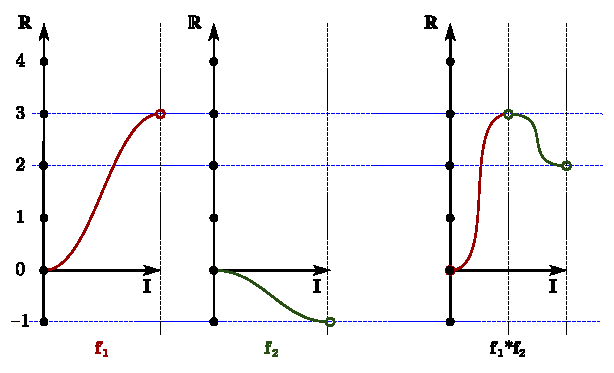
\includegraphics[width=8cm]{./figures/HomT5_1.pdf}
\caption{$S^1$上的回路$f_1$和$f_2$,以及它们的回路积$f_1*f_2$.} \label{HomT5_fig1}
\end{figure}

记按照以上约定所得到的$\tilde{f}(1)$为回路$f$的\textbf{度数},记为$\opn{deg}{f}$.由\autoref{HomT5_fig1} 易知,保基点同伦的回路都有相同的度数,并且$\opn{deg}{f_1*f_2}=\opn{deg}{f_1}+\opn{deg}{f_2}$.

因此,容易得出一维球面的基本群:$\pi_1(S^1)=\mathbb{Z}$.


\end{example}

例子中的讨论是较为严谨的思路,实际上可以直观地把$\pi_1(S^1)$中的各元素(回路类)看成是顺时针或逆时针绕过整个圆周$n$周后回到基点的回路所构成的类,其中$n$是一个整数,因此基本群同构于整数加群.比如说,如果选定逆时针为正方向,那么顺时针旋转$2$圈后回到基点的回路类就对应于$-2$.


\begin{example}{和$S^1$有关的空间中的基本群}
由于$\pi_1(S^1)=\mathbb{Z}$,结合本节所述定理,我们可以轻松计算如下空间的基本群:
\begin{itemize}
\item 甜甜圈空间可以表示为$S^1\times S^1$,因此其基本群为$\pi_1(S^1\times S^1)=\mathbb{Z}\times\mathbb{Z}$.
\item 高维甜甜圈$S^1\times\cdots\times S^1$的基本群是$\mathbb{Z}\times\cdots\times\mathbb{Z}$.
\item 二阶圈图$S^1\vee S^1$(\autoref{Topo9_def1}~\upref{Topo9})的基本群是$\mathbb{Z}*\mathbb{Z}$.
\item 高阶圈图$S^1\vee\cdots\vee S^1$的基本群是$\mathbb{Z}*\cdots*\mathbb{Z}$.
\end{itemize}

\end{example}

\begin{example}{莫比乌斯带的基本群}\label{HomT5_ex1}
莫比乌斯带$M$可以通过强形变收缩(\autoref{HomT2_def1}~\upref{HomT2})来同伦于其中轴线$S^1$,因此莫比乌斯带的基本群和$S^1$一样,都是$\mathbb{Z}$.

理解莫比乌斯带基本群的难点是看出中轴线是其强形变收缩核,为了方便描述如何构造对应的强形变收缩,我们把莫比乌斯带看成射影平面挖去中心的结果,如\autoref{HomT5_fig9} 所示.

\begin{figure}[ht]
\centering
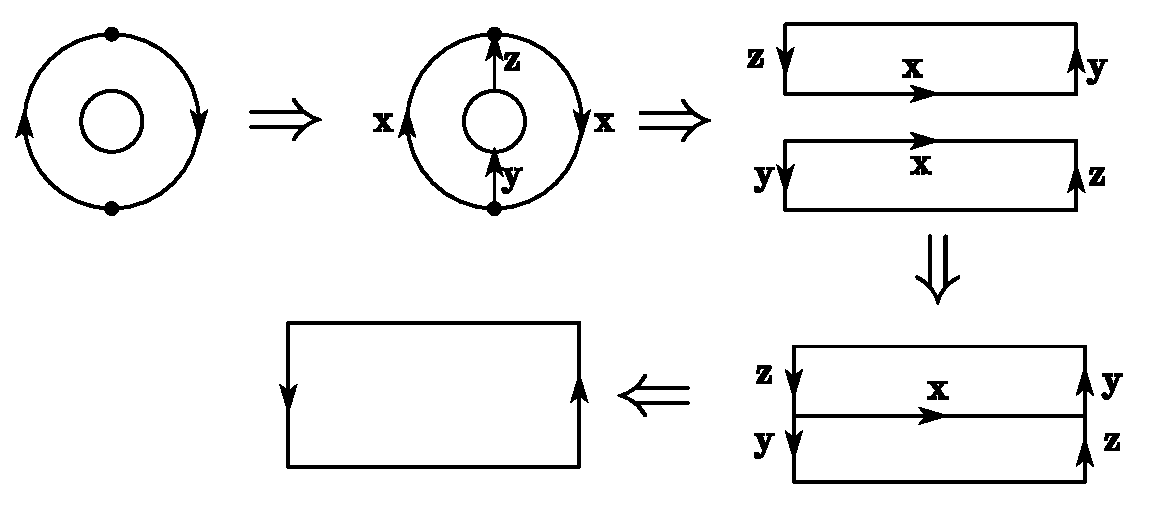
\includegraphics[width=10cm]{./figures/Topo7_9.pdf}
\caption{从射影平面中间挖去一个洞得到莫比乌斯带示意图.详见\textbf{商拓扑}\upref{Topo7}词条.} \label{HomT5_fig9}
\end{figure}

由于射影平面本身可以看成一个圆盘$B^2$的商拓扑空间,我们同样可以把$M$看成圆盘$B^2$挖去中心后再取商拓扑,也就是看成圆环的商拓扑空间.不失一般性地,把这个圆环看成半径为$2$的圆和半径为$1$的圆之间的部分.取映射$f:M\times I\rightarrow M$,其中对于任意$(x, y)\in M, t\in I$,都有$f((x, y), t)= (1+t/(1-\sqrt{x^2+y^2}))(x, y)$,则$f$是一个强形变收缩,其收缩核就是圆环的外边缘;取商拓扑可见,这个外边缘正是莫比乌斯带的中轴线.
\end{example}

\begin{exercise}{莫比乌斯带的强形变收缩}
验证\autoref{HomT5_ex1} 中的$f$是同伦,进而证明它确实是强形变收缩.提示:先考虑未将圆环外边缘的对径点粘合时的情况,再对比考虑粘合后的效果.
\end{exercise}

\begin{exercise}{}
将莫比乌斯带看成一个射影平面挖去中心后的空间.如果将沿着外边缘走了半圈的回路类\footnote{走了半圈就回到了起点,因为对径点粘在一起了.}记为$a\in\pi_1(M)$,那么绕着中心缺口顺时针旋转一周的回路类是$\pi_1(M)$中的哪个元素?

答案是$a^2$.
\end{exercise}



